PHSX611 / EPHX611: Introduction to Quantum Mechanics (Spring 2024)
Homework 8: Final Exam Preparation. See references to appropriate problems in Griffiths. Due: Wed, May 08, 11:59 pm, worth 3.5 points (it gives one extra point to the standard 2.5 pts.)
\begin{homeworkProblem}
	Write down the 1D stationary Schrodinger equation for potential $V(x)=A x^2+\frac{B}{x^2}$. Consider only $x>0, A>0, B>0$. Sketch this potential. Find the minimal energy at which the Schrodinger equation will have at least one solution. Comment on the type of spectra for each value of energy. ( $0.5 \mathrm{pt}$).
	\begin{callout}{Solution:}

		\vspace{0.25cm} (1) \begin{align*}
			\hat{H} \ket{\psi}                                                                                                         & = i \hbar \ket{\psi} \\
			-\frac{\hbar^{2}}{2m} \frac{ \partial^{2} \ket{\psi} }{ \partial x^{2} } + \left( Ax^{2}+\frac{B}{x^{2}} \right)\ket{\psi} & =i\hbar \ket{\psi}
		\end{align*}

		(2)
		\begin{center}
			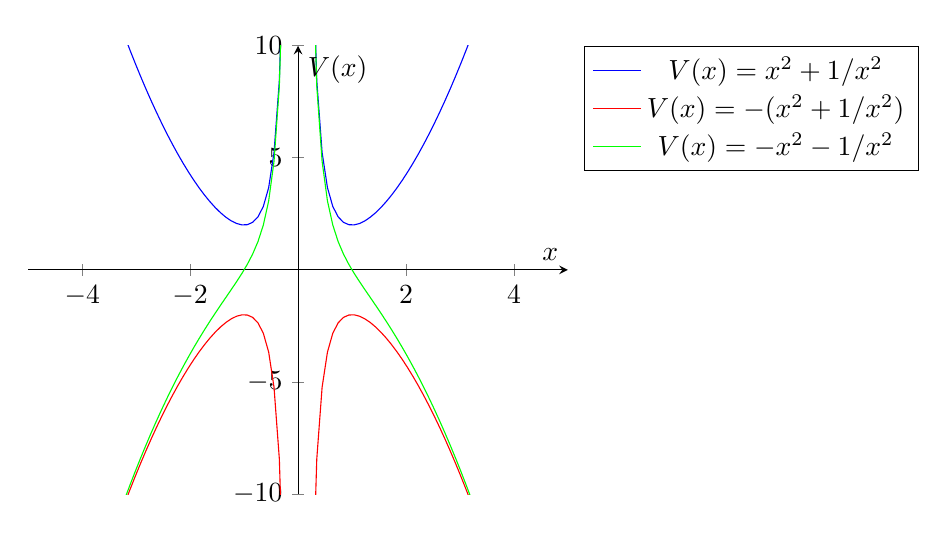
\begin{tikzpicture}
				\begin{axis}[
						xlabel=$x$,
						ylabel=$V(x)$,
						xmin=-5, xmax=5,
						ymin=-10, ymax=10,
						samples=100,
						domain=-4.9:4.9,
						legend pos=outer north east,
						axis lines=middle,
						minor tick num=0
					]
					\addplot[blue] {x^2 + 1/x^2};
					\addlegendentry{$V(x) = x^2 + 1/x^2$}
					\addplot[red] {-(x^2 + 1/x^2)};
					\addlegendentry{$V(x) = -(x^2 + 1/x^2)$}
					\addplot[green] {-x^2 + 1/x^2};
					\addlegendentry{$V(x) = -x^2 - 1/x^2$}
				\end{axis}
			\end{tikzpicture}
		\end{center}

		\newpage (3) We can bound the minimum energy based on the fact that the energy always exceeds the minimum of the potential. Finding the extrema of the potential:

		\begin{gather*}
			\frac{d}{dx}\left( Ax^{2}+\frac{B}{x^{2}} \right)=2Ax-\frac{2B}{x^3}=0 \implies 2Ax^4-2B=0 \\
			x^2=u; \quad u=\pm\sqrt{\frac{B}{A}}                                                       \\
			x=\pm\left( \frac{B}{A} \right)^{1/4},~x=\pm i\left( \frac{B}{A} \right)^{1/4}
		\end{gather*}

		Of course, if these are concave down then there is no minimum energy, and instead the critcal point tells us when solutions become continuous. We can check concavity with a little more calculus:

		\begin{align*}
			\frac{d^{2}}{dx^{2}}\left( Ax^{2}+\frac{B}{x^{2}} \right) = 2A+\frac{6B}{x^4} = 0 \\
			u=x^{2};\quad 2Au^{2}+6B=0 \implies \dots                                         \\
			x=\pm\left( \frac{3B}{4A} \right)^{1/4}\pm\left( \frac{3B}{4A} \right)^{1/4}i
		\end{align*}

		A closed form solution to the shrödinger equation is necessary to get a more precise bound on the allowed energies, just like in the harmonic oscillator or finite square well problems.

	\end{callout}
\end{homeworkProblem}

\newpage \begin{homeworkProblem}
	How would you calculate the average bond length of an electron and proton in a hydrogen atom at a given n? For that, you may want to solve Problem 4.15. (0.5 pts.)
	\begin{callout}{Solution:}

		In general, applying an operator to the wavefunction of the hydrogen atom involves nothing new. For an arbitrary $n$, the average bond length is  $\braket{ R_{n\ell}(r) | \hat{r} |R_{n\ell}(r)}$. I had originally reasoned that the solution Would be $\sqrt{ \braket{ R_{n\ell}(r) | \hat{r}^{2}|R_{n\ell}(r)} }$, however this is in fact the root mean square which is a different thing entirely, apparently.

		Obviously there are relatively complicated polynomials involved in the wavefunction of the hydrogen atom, and while some research has led me to believe it is (probably) possible to analytically integrate the squares of these using their generating sum, it is far too daunting a task to do so. Instead I'll simply pick my favorite quantum numbers: $n=2,~\ell=1,~m=1$. Note that the time component cancels due to the complex conjugate.

		\begin{align*}
			R_{21}(r)             & = \frac{1}{2 \sqrt{ 6 }}a^{-2/3} \left( \frac{r}{a} \right) e^{-r/2a} \\
			Y_1^{1}(\theta, \phi) & = -\sqrt{ \frac{3}{8\pi} } \sin\theta e ^{i\phi}                      \\
			\psi(r, \theta, \phi) & = R_{21}(r) Y_1^1(\theta,\phi)
		\end{align*}

		$$
			\underset{\text{(all space)}}{\iiint} \left( -\frac{1}{8 \sqrt{ \pi }}a^{-2/3} \left( \frac{r}{a} \right) e^{-r/2a}\sin\theta e ^{i\phi} \right) r \left( -\frac{1}{8 \sqrt{ \pi }}a^{-2/3} \left( \frac{r}{a} \right) e^{-r/2a}\sin\theta e ^{-i\phi}  \right) r^2 \sin \theta ~dr~d\phi~d\theta
		$$
		Which simplifies to
		$$\frac{1}{64\pi a^{10/3}}\underset{\text{(all space)}}{\iiint}
			e^{-r/a}r^5\sin ^3\theta ~d\theta ~dr ~d\phi$$

		\begin{gather*}
			\frac{1}{64\pi a^{10/3}}\left( \int_{0}^{\pi} \sin ^{3}\theta\,d\theta  \right)\left( \int_{0}^{\infty} e^{-r/a}r^{5}\,dr  \right)\left( \int_{0}^{2\pi} d\phi \right) \\
			\frac{1}{64\pi a^{10/3}}\left( \int_{0}^{\pi} (1-\cos ^{2}\theta)\sin \theta\,d\theta  \right)\left( \int_{0}^{\infty} e^{-ur} \frac{ \partial^{5} }{ \partial r^{5} }  \,du  \middle)\right|_{u=\frac{1}{a}}\left(2\pi\right) \\
			\frac{1}{64\pi a^{10/3}}\left( \int_{-1}^{1} (1-w^{2})\,dw  \right) \frac{d^{5}}{du^{5}} \left( \int_{0}^{\infty} e^{-ur}  \,du  \middle)\right|_{u=\frac{1}{a}}\left(2\pi\right) \\
			\frac{1}{64\pi a^{10/3}}\left( \frac{4}{3}  \right) \frac{d^{5}}{du^{5}} \left( \frac{1}{u}  \middle)\right|_{u=\frac{1}{a}}\left(2\pi\right) \\
			\frac{1}{64\pi a^{10/3}}\left( \frac{4}{3}  \right) (120a^{6}\left)(2\pi\right) \\
			5a^{\frac{8}{3}} \mathrm{~m}
		\end{gather*}

	\end{callout}
\end{homeworkProblem}

\newpage \begin{homeworkProblem}
	Same as previous, calculate $\langle x\rangle,\left\langle x^2\right\rangle,\left\langle r^2\right\rangle$. ( 0.5 pts.)
	\begin{callout}{Solution:}

		\begin{enumerate}[(1)]
			\item $\langle x \rangle$:
			      After realizing I can no longer explot symmetry to solve this I have decided my favorite state is no longer the one I mentioned. The integral goes:
			      \begin{callout}{Solution:}

				      \begin{gather*}
					      \frac{1}{64\pi a^{10/3}}\underset{\text{(all space)}}{\iiint}(e^{-r/a}r^4\sin^3\theta)(r\sin \theta \cos \phi) ~d\theta ~dr ~d\phi \\
					      \frac{1}{64\pi a^{10/3}} \left( \int_{0}^{\pi} \sin ^{4}\theta\,d\theta  \right)\left( \int_{0}^{\infty}e^{-r/a}r^{5} \,dr  \right)\left( \int_{0}^{2\pi} \cos \phi\,d\phi  \right) \\
					      \frac{1}{64\pi a^{10/3}} \left( \int_{0}^{\pi} (1-\cos ^{2}\theta)(1-\cos ^{2}\theta)\,d\theta  \right)\left( \int_{0}^{\infty} e^{-ur}\frac{ \partial^{5} }{ \partial r^{5} } \,dr \middle)\right|_{u=\frac{1}{a}}\left( 0\right) \\
					      =0
				      \end{gather*}
				      Thankfully the $\hat{x}$ operator forces this to zero, however the same will not be true for the square.

			      \end{callout}
			\item $\langle x^2 \rangle$:
			      \begin{gather*}
				      \frac{1}{64\pi a^{10/3}}\underset{\text{(all space)}}{\iiint}(e^{-r/a}r^4\sin^3\theta)(r\sin \theta \cos \phi) ~d\theta ~dr ~d\phi \\
				      \frac{1}{64\pi a^{10/3}} \left( \int_{0}^{\pi} \sin ^{4}\theta\,d\theta  \right)\left( \int_{0}^{\infty}e^{-r/a}r^{6} \,dr  \right)\left( \int_{0}^{2\pi} \cos ^{2} \phi\,d\phi  \right) \\
				      \frac{1}{64\pi a^{10/3}} \left( \int_{0}^{\pi} \sin ^{4}\theta\,d\theta  \right)\left( \int_{0}^{\infty} e^{-ur}\frac{ \partial^{5} }{ \partial r^{5} } \,dr \middle)\right|_{u=\frac{1}{a}}\left(\int_{0}^{2\pi} \frac{1}{2} (1-\sin(2\theta)) \,d\phi \right) \\
				      \frac{1}{64\pi a^{10/3}} \left( \int_{0}^{\pi} \sin ^{4}\theta\,d\theta   \right) \frac{d^{5}}{dr^{5}} \left( \frac{1}{u} \middle)\right|_{u=\frac{1}{a}}\left(2\pi\right) \\
				      \frac{1}{64\pi a^{10/3}} \left(\frac{3\pi}{8}\right)(120a^6)\left(2\pi\right) \\
				      \frac{45\pi a^{\frac{8}{3}}}{32} \mathrm{~m^{2}}
			      \end{gather*}
			\item $\langle r^2 \rangle$:
			      \begin{gather*}
				      \frac{1}{64\pi a^{10/3}}\underset{\text{(all space)}}{\iiint}e^{-r/a}r^6\sin ^3\theta ~d\theta ~dr ~d\phi                                                                                                         \\
				      \frac{1}{64\pi a^{10/3}}\int_{0}^{\pi} \sin ^{3}\theta\,d\theta \int_{0}^{\infty} e^{-r/a}r^{6}\,dr \int_{0}^{2\pi} d\phi                                                                                            \\
				      \frac{1}{64\pi a^{10/3}}\left( \int_{0}^{\pi} (1-\cos ^{2} \theta)\sin \theta\,d\theta \right) \left( \int_{0}^{\infty} -e^{-ur} \frac{ \partial^{6} }{ \partial u^{6} } \,dr \middle)\right|_{u=\frac{1}{a}} (2\pi) \\
				      \frac{1}{64\pi a^{10/3}}\left( \int_{-1}^{1} 1-w^{2}\,dw \right) \frac{d^{6}}{du^{6}}\left( \int_{0}^{\infty} -e^{-ur} \,dr \middle)\right|_{u=\frac{1}{a}} (2\pi)                                                   \\
				      \frac{1}{64\pi a^{10/3}}\left( \frac{4}{3}\right) \frac{d^{6}}{du^{6}}\left(\frac{1}{u}\middle)\right|_{u=\frac{1}{a}} (2\pi)                                                                                        \\
				      \frac{1}{64\pi a^{10/3}}\left( \frac{4}{3}\right) \left(\frac{720}{u^7}\middle)\right|_{u=\frac{1}{a}} (2\pi)                                                                                                        \\
				      \frac{1}{64\pi a^{10/3}}\left( \frac{4}{3}\right) \left(720a^7\right) (2\pi)                                                                                                                                         \\
				      30a^{\frac{11}{3}} \mathrm{~m^2}
			      \end{gather*}
		\end{enumerate}

	\end{callout}
\end{homeworkProblem}

\newpage \begin{homeworkProblem}
	Calculate the most probable value of $r$ for the hydrogen atom. Is it different in the ground state and the first excited state? Solve Problem 4.16. ( 0.5 pts.)
	\begin{callout}{Solution:}

		Probability of radius is given simply by the PDF of the radial component:
		\begin{gather*}
			\iiint \left(\frac{1}{\sqrt{\pi a^3}} e^{-r / a} e^{i E_1 t / \hbar}\right)\left(\frac{1}{\sqrt{\pi a_0^3}} e^{-r / a} e^{-i E_1 t / \hbar}\right) d^{3}r \\
			\iiint \frac{1}{\pi a^3} e^{-2 r / a} (r^{2}\sin \theta~dr~d\theta~d\phi) \\
			\frac{1}{\pi a^{3}} \left( \int_0^{2\pi} d\phi \right)\left( \int e^{-r/a}r^{2}\,dr \right)\left( \int_0^{\pi} \sin \theta\,d\theta  \right) \\
			\frac{1}{\pi a^{3}} (2\pi) \left( 1-\frac{r}{a} \right)(2)
		\end{gather*}
		As we'd normally integrate to find probability between $a$ and $b$, this is already the derivative. Setting this equal to find extrema clearly gives solutions $\{ 0,~a \}$. This will also be different in different energy levels.


	\end{callout}
\end{homeworkProblem}

\newpage \begin{homeworkProblem}
	Derive the formula and calculate the expectation value of the potential energy of the hydrogen atom. Does it depend on time? Solve Problem 4.18. ( 0.5 pts.)
	\begin{callout}{Solution:}

		Doing this once with our favorite quantum numbers, where again the time will cancel out.

		\begin{gather*}
			\frac{1}{64\pi a^{10/3} } \underset{\text{(all space)}}{\iiint} -\frac{e^2}{4\pi\epsilon_{0}r}(e^{-r/a}r^4\sin ^3\theta) ~d\theta ~dr ~d\phi \\
			=-\frac{e^{2}}{256\pi^{2} \epsilon_{0} a^{10/3}} \int_{0}^{2\pi} d\phi \int_{0}^{\infty} e^{-r/a}r^3\,dr \int_{0}^{2\pi} \sin ^{3}\theta\,d\theta \\
			=-\frac{e^{2}}{256\pi^{2} \epsilon_{0} a^{10/3}}(2\pi)(6a^{4})\left( -\frac{4}{3} \right) \\
			=\frac{e^2a^{\frac{2}{3}}}{16\pi \epsilon_{0}}~\textrm{eV}
		\end{gather*}

		\newpage The integral gets a little spicier using the linear combination in problem 4.18, as $\phi$ will no longer vanish. I'll just skip to the integral again:
		\tiny $$\int_0^\pi \int_0^{2 \pi} \int_0^{\infty}\left[+\frac{i}{\sqrt{32 \pi ^5}}(r \sin \theta \sin \phi) e^{-r /\left(2 \right)} \cancel{e^{i E_2 t / \hbar}}\right]\left(-\frac{e^2}{4 \pi \epsilon_0 r}\right)\left[-\frac{i}{\sqrt{32 \pi ^5}}(r \sin \theta \sin \phi) e^{-r /\left(2 \right)} \cancel{e^{-i E_2 t / \hbar}}\right]\left(r^2 \sin \theta d r d \phi d \theta\right)$$ \normalsize

		\begin{gather*}
			-\frac{e^{2}}{128\pi^{2} \epsilon_{0}a_{0}^{5}} \int_{0}^{\pi} \sin ^{3}\theta\,d\theta \int_{0}^{2\pi} \sin ^{2}\phi\,d\phi \int_{0}^{\infty} r^{3}e^{-r/a}\,dx \\
			-\frac{e^{2}}{128\pi^{2} \epsilon_{0}a_{0}^{5}} \left( \int_{0}^{\pi}(1-\cos ^{2}\theta)\sin \theta \,d\theta  \right)\left( \int_{0}^{2\pi} \frac{1}{2}(1-\cos(2\phi))\,d\phi  \right)(-6a^{4}) \\
			-\frac{e^{2}}{128\pi^{2} \epsilon_{0}a_{0}^{5}}\left( \int_{\cos0}^{\cos \pi}(1-w^{2}) \,dw  \right)(\pi)(-6a^{4}) \\
			-\frac{e^{2}}{128\pi^{2} \epsilon_{0}a_{0}^{5}}\left(\frac{4}{3}\right)(\pi)(-6a^{4}) \\
			\frac{e^2}{16\pi a\epsilon_{0}}~\textrm{eV}
		\end{gather*}


	\end{callout}
\end{homeworkProblem}

\newpage \begin{homeworkProblem}
	Derive a spherical harmonic $Y_3^3(\theta, \phi)$. How would you normalize it? Use Lectures $\mathbf{3 4 , 3 5}$ and find a way to get to other harmonics with $l=3$. ( 0.5 pts.)
	\begin{callout}{Solution:}

		For the sake of my own studying, I'll derive spherical harmonics starting from the separated angular equation:


		$$\phi(r,\theta,\phi)=R(r)Y(\theta,\phi):$$
		$$\left\{ \frac{1}{R} \frac{d}{dr}\left( r^{2} \frac{dR}{dr} \right)-\frac{2mr^{2}}{\hbar^{2}}[V(r)-E] \right\}+\frac{1}{Y}\left\{ \frac{1}{\sin \theta} \frac{ \partial }{ \partial \theta } \left( \sin \theta \frac{ \partial Y }{ \partial \theta }  \right)+\frac{1}{\sin ^{2}\theta} \frac{ \partial^{2}Y }{ \partial \phi^{2} }  \right\} = 0$$
		Our separation constant is $\ell(\ell+1)$:
		$$\to \sin\theta \frac{ \partial }{ \partial \theta } \left( \sin \theta \frac{ \partial Y }{ \partial \theta }  \right)+\frac{ \partial^{2}Y }{ \partial \phi^{2} } =-\ell(\ell+1)\sin ^{2}\theta Y$$

		Separating further gives:
		$$\left\{ \frac{1}{\Theta}\left( \sin \theta  \frac{d}{d\theta}\left( \sin \theta  \frac{d\Theta}{d\theta} \right) \right)+\ell(\ell+1)\sin ^{2}\theta\right \}+ \left\{ \frac{1}{\Phi} \frac{d^{2}\Phi}{d\phi^{2}}\right \}=m^{2})$$

		Polar angle is easy:
		$$\frac{d^{2}\Phi}{d\phi^{2}}=-m^{2}\Phi\implies \Phi(\phi)=e^{im\phi}$$

		Azimuthal is a lot harder, but it gives:
		$$\Theta(\theta)=AP_{\ell}^{m}(\cos \theta); \qquad \begin{array}{rl}
				P_{\ell}^{m}(x)\hspace{-0.3cm} & =(-1)^{m}(1-x^{2})^{m/2}\left( \frac{d}{dx} \right)^{m}P_{\ell}(x),         \\
				P_{\ell}(x)\hspace{-0.3cm}     & =\frac{1}{2^{\ell}\ell!} \left( \frac{d}{dx} \right)^{\ell}(x^{2}-1)^{\ell}
			\end{array}$$

		In this case $P_3=\frac{1}{2}(5x^3-3x)$ and $Y_3^3=A \sin^3\theta e^{3i\phi}$. Normalizing using trig equalities and substitution (really there's nothing special about the normalization of this function) gives:

		$$Y_3^3(\theta,\phi)=-\sqrt{ \frac{35}{64\pi} }\sin^3\theta e^{3i\phi}$$

		We can apply ladder operators to jump between $m$:

		$$Y_3^2(\theta,\phi)=\frac{1}{\sqrt{ 6 }}\hat{\ell}_{-}Y_{3}^{3}(\theta,\phi), \qquad \hat{\ell}_{-}=-e^{-i\phi}\left\{  -i\cot \theta \frac{ \partial }{ \partial \phi } \right\}$$

	\end{callout}
\end{homeworkProblem}

\newpage \begin{homeworkProblem}
	Calculate eigenvalues and eigenvectors for the Hamiltonian of a spin $1 / 2$ particle in the magnetic field that is applied in the $\mathrm{y}-\mathrm{z}$ plane. Derive a general formula for operator $(\hat{\vec{\sigma}} \cdot \vec{n})$ for eigenvalues and eigenvectors. Which basis are you using to write down matrix $(\hat{\vec{\sigma}} \cdot \vec{n})$ ? Use Lectures 36 - 38. ( 0.5 pts.)
	\begin{callout}{Solution:}

		In polar coordinates:
		$$\mathbf{n}=(r\sin \theta \sin \phi,\, r\sin \theta \cos \phi,\,r\cos \phi)$$
		Restricting $\phi$ to 0 gives us the two dimensional subspace corresponding to the $y$-$z$ plane. Computing $\braket{ \hat{\mathbf{\sigma}} | \mathbf{n}}$ gives.
		\begin{gather*}
			\begin{pmatrix} 0 & 1 \\ 1 & 0 \end{pmatrix}\sin \theta \sin \phi+\begin{pmatrix}0 & -i \\ i & 0\end{pmatrix}\sin \theta \cos \phi+\begin{pmatrix} 1 & 0 \\ 0 & -1 \end{pmatrix} \cos \theta \\
			=\begin{pmatrix} \cos \theta & \sin \theta e^{-i\phi}\\ \sin \theta e^{-i\phi} & -\cos \theta \end{pmatrix}
		\end{gather*}
		It's worth mentioning where $\hat{\sigma}$ came from. We already know that in the basis of spin 1/2:
		\begin{gather}
			\hat{s}_{\pm}\ket{s~m}= \hbar \sqrt{ s(s+1)-m(m\pm1) } \ket{ s~(m\pm1)} \\
			\hat{s}_{z}\ket{s~m} =m\ket{s~m}
		\end{gather}

		For the sake of example, the matrix form of $\hat{s}_{z}$ on our basis is found by applying the operator to each index of the matrix, $\braket{ i | \hat{s}_{z}|j}$:
		$$\hat{s}_{z}=\begin{pmatrix}
				\frac{1}{2} & 0           \\
				0           & \frac{1}{2}
			\end{pmatrix}$$


		We can express the $x$-$y$ components
		$$\hat{s}_{\pm}=\hat{s}_{x}\pm i\hat{s}_{y} \implies \left\{\begin{array}{rl}
				\hat{s}_{x}\hspace{-0.3cm} & =\frac{1}{2}(s_{+}+s_{-})   \\
				\hat{s}_{y}\hspace{-0.3cm} & = \frac{1}{2i}(s_{+}-s_{-})
			\end{array}\right.$$

		Where we have matrix representations of the raising and lowering operators:

		$$\hat{s}_{+}=\begin{pmatrix}0 & 1 \\0 & 0\end{pmatrix}, \qquad \hat{s}_{-}=\begin{pmatrix}0 & 0\\1 & 0\end{pmatrix}$$

		Which in turn gives us scalar multiples of these matrices:

		$$\hat{s}_{x}= \frac{1}{2}\begin{pmatrix} 0 & 1 \\ 1 & 0\end{pmatrix}, \qquad
			\hat{s}_{y}=\begin{pmatrix} 0 & -i \\ i & 0 \end{pmatrix}, \qquad
			\hat{s}_{z}=\frac{1}{2}\begin{pmatrix}1 & 0\\0 & 1\end{pmatrix}$$
	\end{callout}
\end{homeworkProblem}
